\begin{frame}
  \frametitle{Hybrid $S_N$-Diffusion Method: 1-D Neutronics Eigenvalue Simulations}
  \textbf{1-D Neutronics Model Geometries}
  \begin{figure}[htb!]
    \centering
    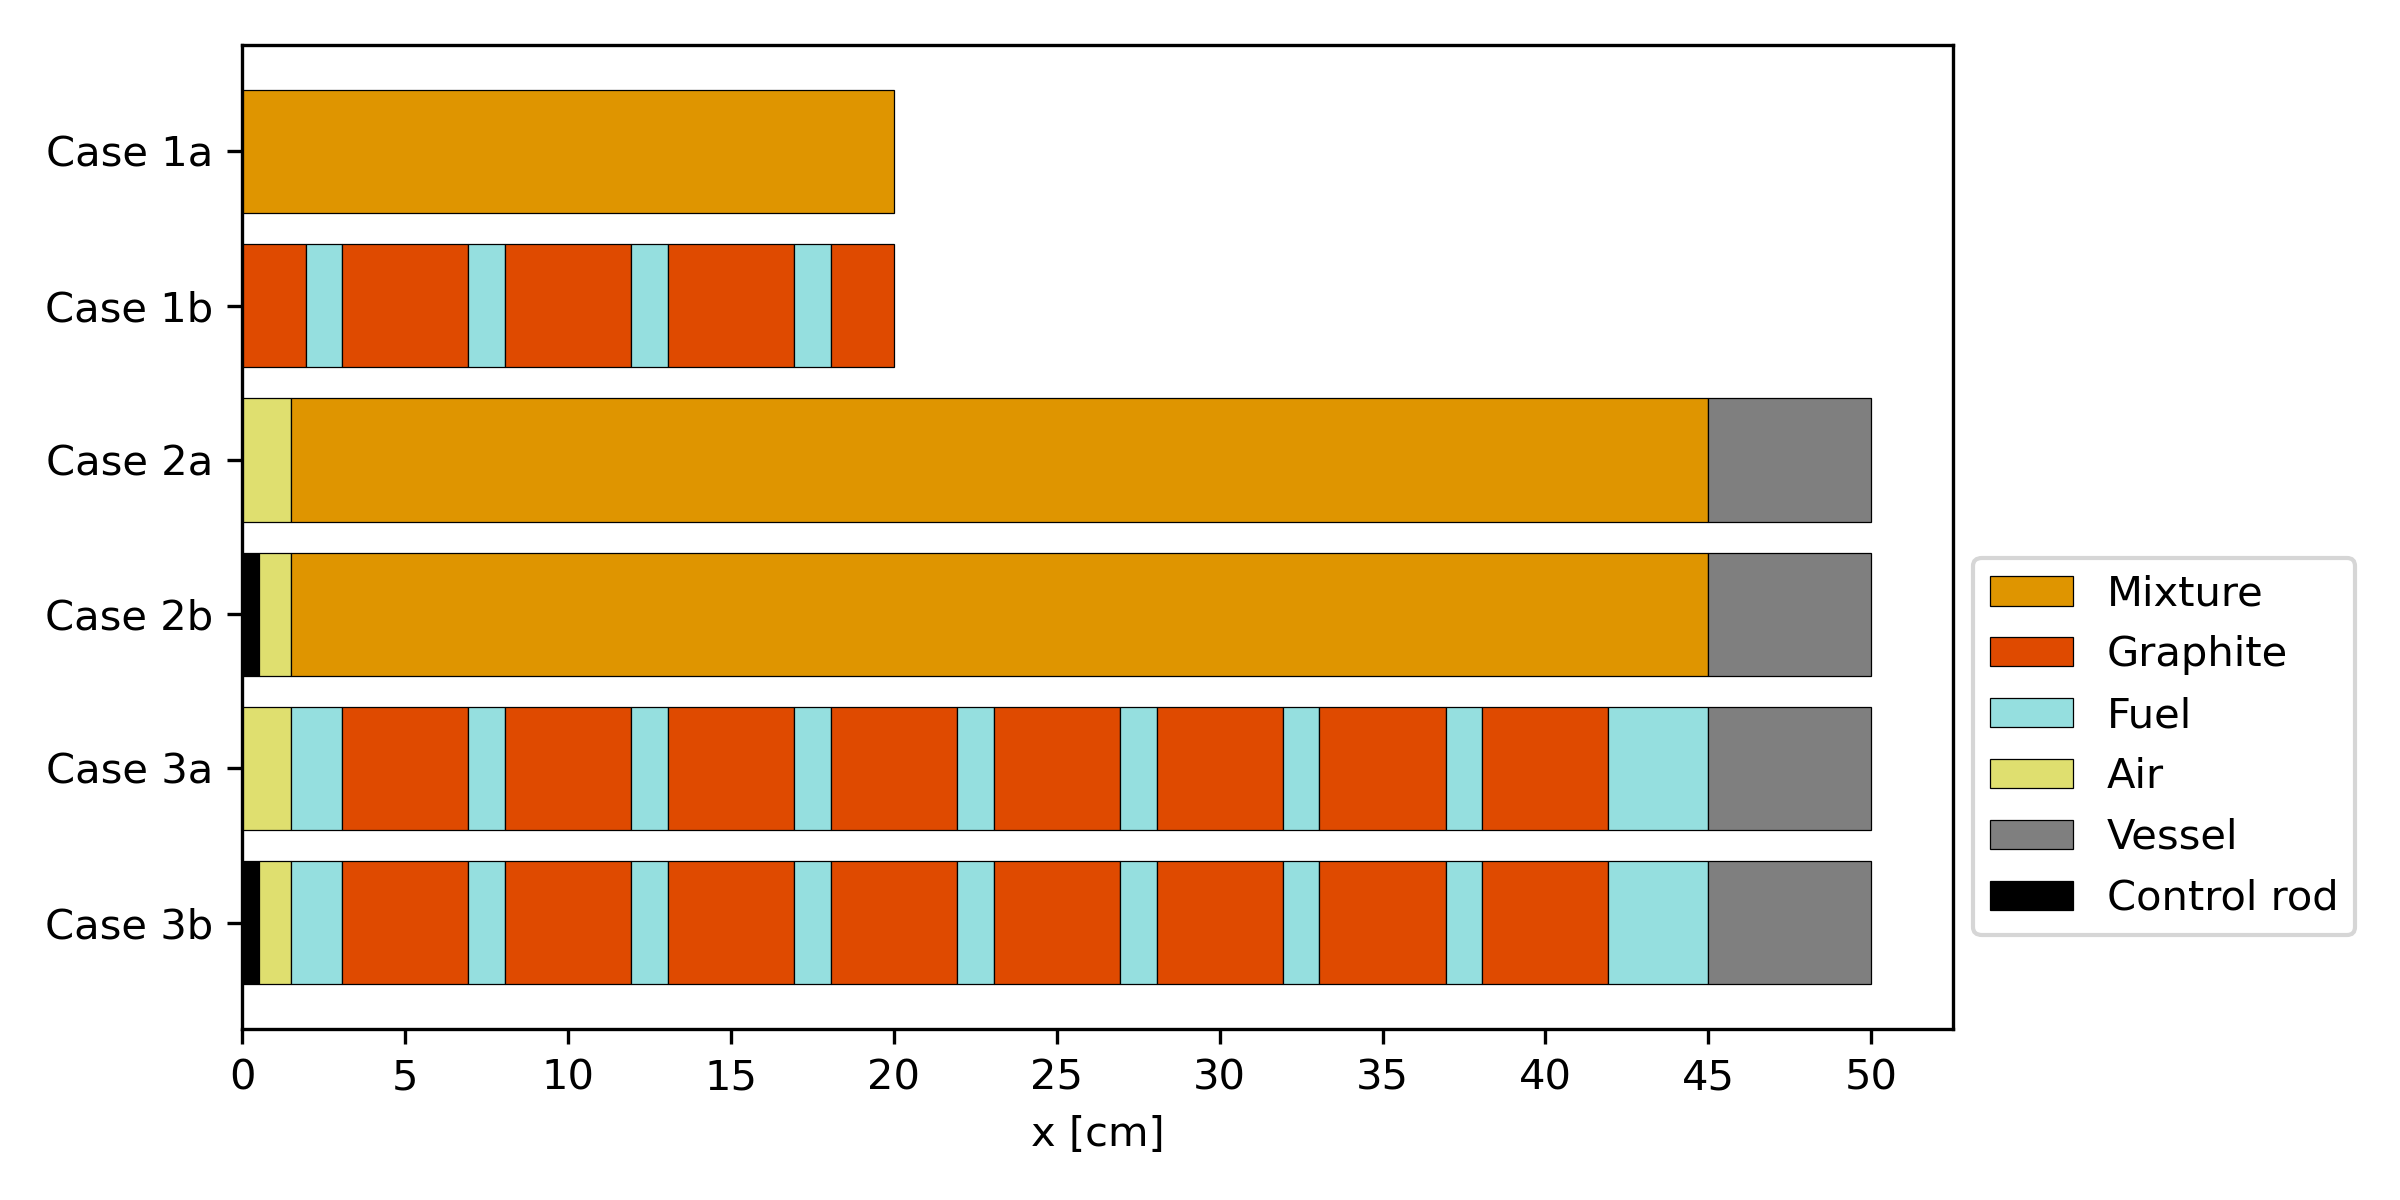
\includegraphics[width=0.9\columnwidth]{case-geometry}
    \caption{Geometries of the 1-D test cases. The material labeled ``mixture'' represents a
      homogeneous mixture of fuel and graphite at a ratio of 22.5\%-77.5\% by volume. All geometries
      have reflective boundary conditions on the boundary at $x=0$ cm. The right-side boundaries are
      reflective for Cases 1a and 1b, and vacuum for Cases 2a, 2b, 3a, and 3b.}
    \label{fig:case-geom}
  \end{figure}
\end{frame}

\begin{frame}
  \frametitle{Hybrid $S_N$-Diffusion Method: 1-D Neutronics Eigenvalue Simulations}
  \begin{columns}
    \column{5.5cm}
    \textbf{1-D Neutronics Model Setup}
    \vspace{.2cm}

    \begin{itemize}
      \item Material compositions derived from the MSRE design
      \item Reduced gadolinium content in control rod to reduce rod worth from 50000 pcm to 20000 pcm
      \item Eight neutron energy groups
      \item Group constants generated using OpenMC with up to 2nd-order Legendre expansions of scattering
        matrices
      \item Uniform temperature at 900 K
    \end{itemize}
    \column{5.5cm}
    \begin{table}[h]
      \centering
      \caption{Neutron energy group structure in this work. Originally devised by Jaradat
      \cite{jaradat_development_2021-1}.}
      \begin{tabular}{r S}
        \toprule
        Group & {Upper energy bound [eV]} \\
        \midrule
        1 & 2.000$\times 10^7$ \\
        2 & 1.353$\times 10^6$ \\
        3 & 6.734$\times 10^4$ \\
        4 & 9.118$\times 10^3$ \\
        5 & 1.487$\times 10^2$ \\
        6 & 4.000$\times 10^0$ \\
        7 & 6.250$\times 10^{-1}$ \\
        8 & 8.000$\times 10^{-2}$ \\
        \bottomrule
      \end{tabular}
      \label{table:energy-group}
    \end{table}
  \end{columns}
\end{frame}

\begin{frame}
  \frametitle{Hybrid $S_N$-Diffusion Method: 1-D Neutronics Eigenvalue Simulations}
  \textbf{1-D Neutronics Model Numerical Solvers}
  \vspace{.2cm}

  All 1-D cases ran on each of the following numerical solvers:
  \begin{enumerate}
    \item OpenMC in continuous energy mode (OpenMC-CE)
    \item OpenMC in multigroup mode (OpenMC-MG)
    \item Standard neutron diffusion method (Moltres \& Python)
    \item $S_8$ method (Moltres \& Python)
    \item Hybrid $S_8$-diffusion method (Moltres \& Python)
  \end{enumerate}
  \vspace{.2cm}

  \textbf{Reactivity \& Reactivity Difference}
  \begin{gather}
    \mbox{Reactivity } \rho \equiv \frac{k_\text{eff}-1}{k_\text{eff}}.
  \end{gather}
  \begin{gather}
    \Delta\rho = \rho_1 - \rho_2 =
    \frac{k_{\text{eff},1}-k_{\text{eff},2}}{k_{\text{eff},1}k_{\text{eff},2}}.
  \end{gather}
\end{frame}

\begin{frame}
  \frametitle{Hybrid $S_N$-Diffusion Method: 1-D Neutronics Eigenvalue Simulations}
  \textbf{1-D Neutronics Model Reactivity Results}
  \begin{figure}[h]
    \centering
    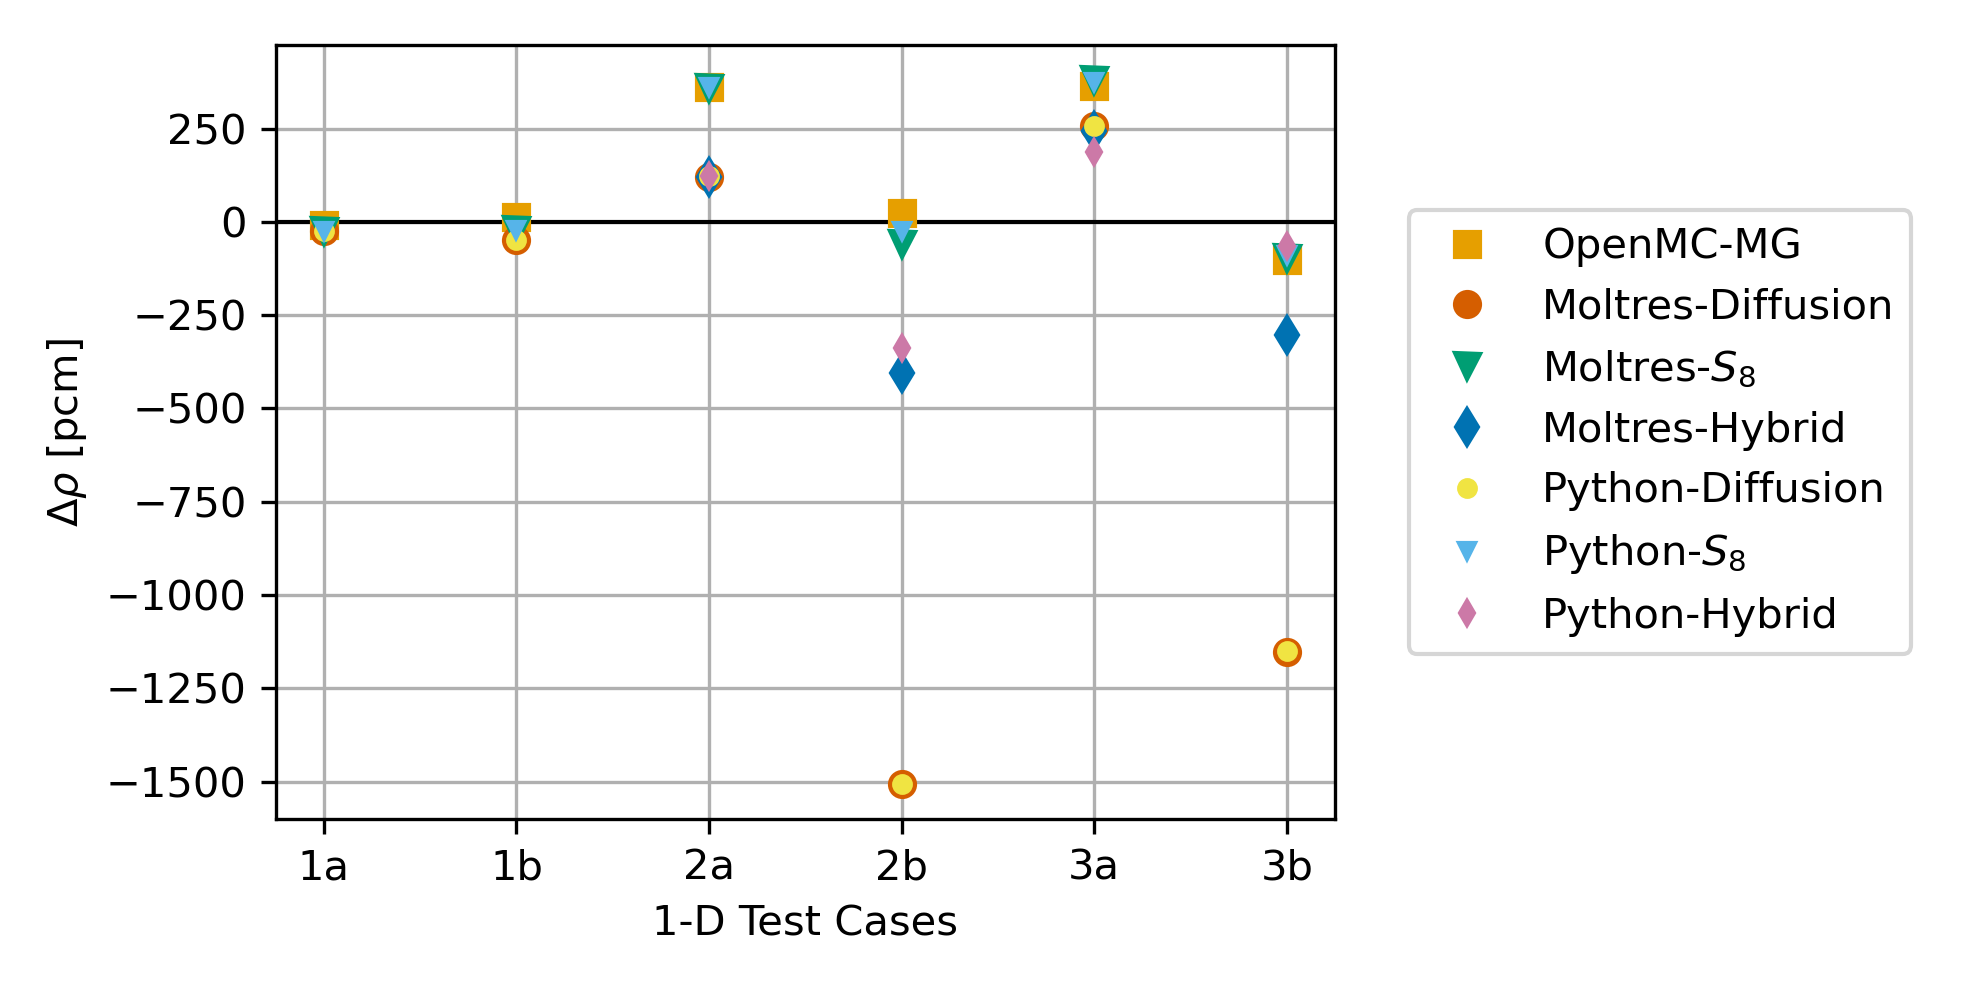
\includegraphics[width=\columnwidth]{rho}
    \caption{Difference in reactivity $\rho$ of all neutronics methods investigated relative
    to OpenMC-CE.}
    \label{fig:1d-rho}
  \end{figure}
\end{frame}

\begin{frame}
  \frametitle{Hybrid $S_N$-Diffusion Method: 1-D Neutronics Eigenvalue Simulations}
  \textbf{1-D Neutronics Model Control Rod Worth Results}
  \begin{figure}[h]
    \centering
    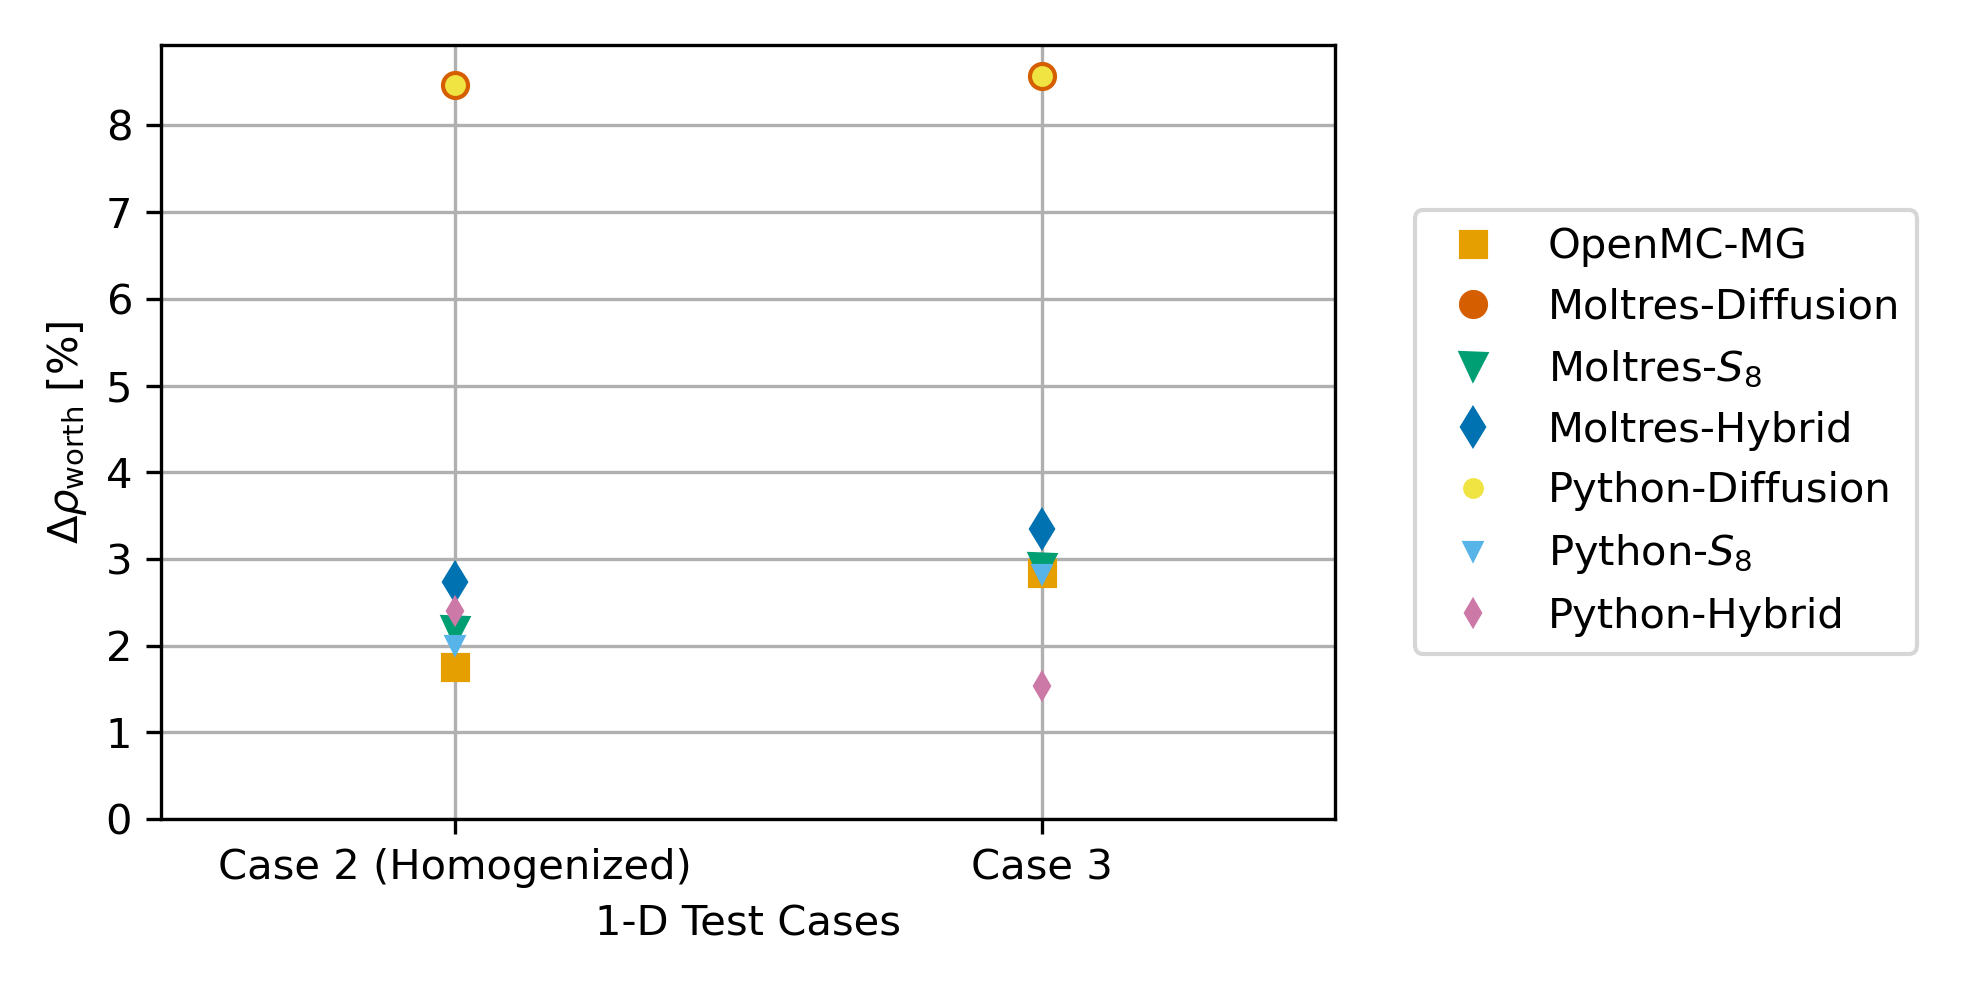
\includegraphics[width=\columnwidth]{worth}
    \caption{Percentage difference in rod worth for Cases 2 and 3 of all neutronics methods
    investigated relative to OpenMC-CE.}
    \label{fig:1d-worth}
  \end{figure}
\end{frame}

\begin{frame}
%  \frametitle{Hybrid $S_N$-Diffusion Method: 1-D Neutronics Eigenvalue Simulations}
  \begin{columns}
    \column{5.5cm}
    \begin{figure}[htb!]
      \centering
      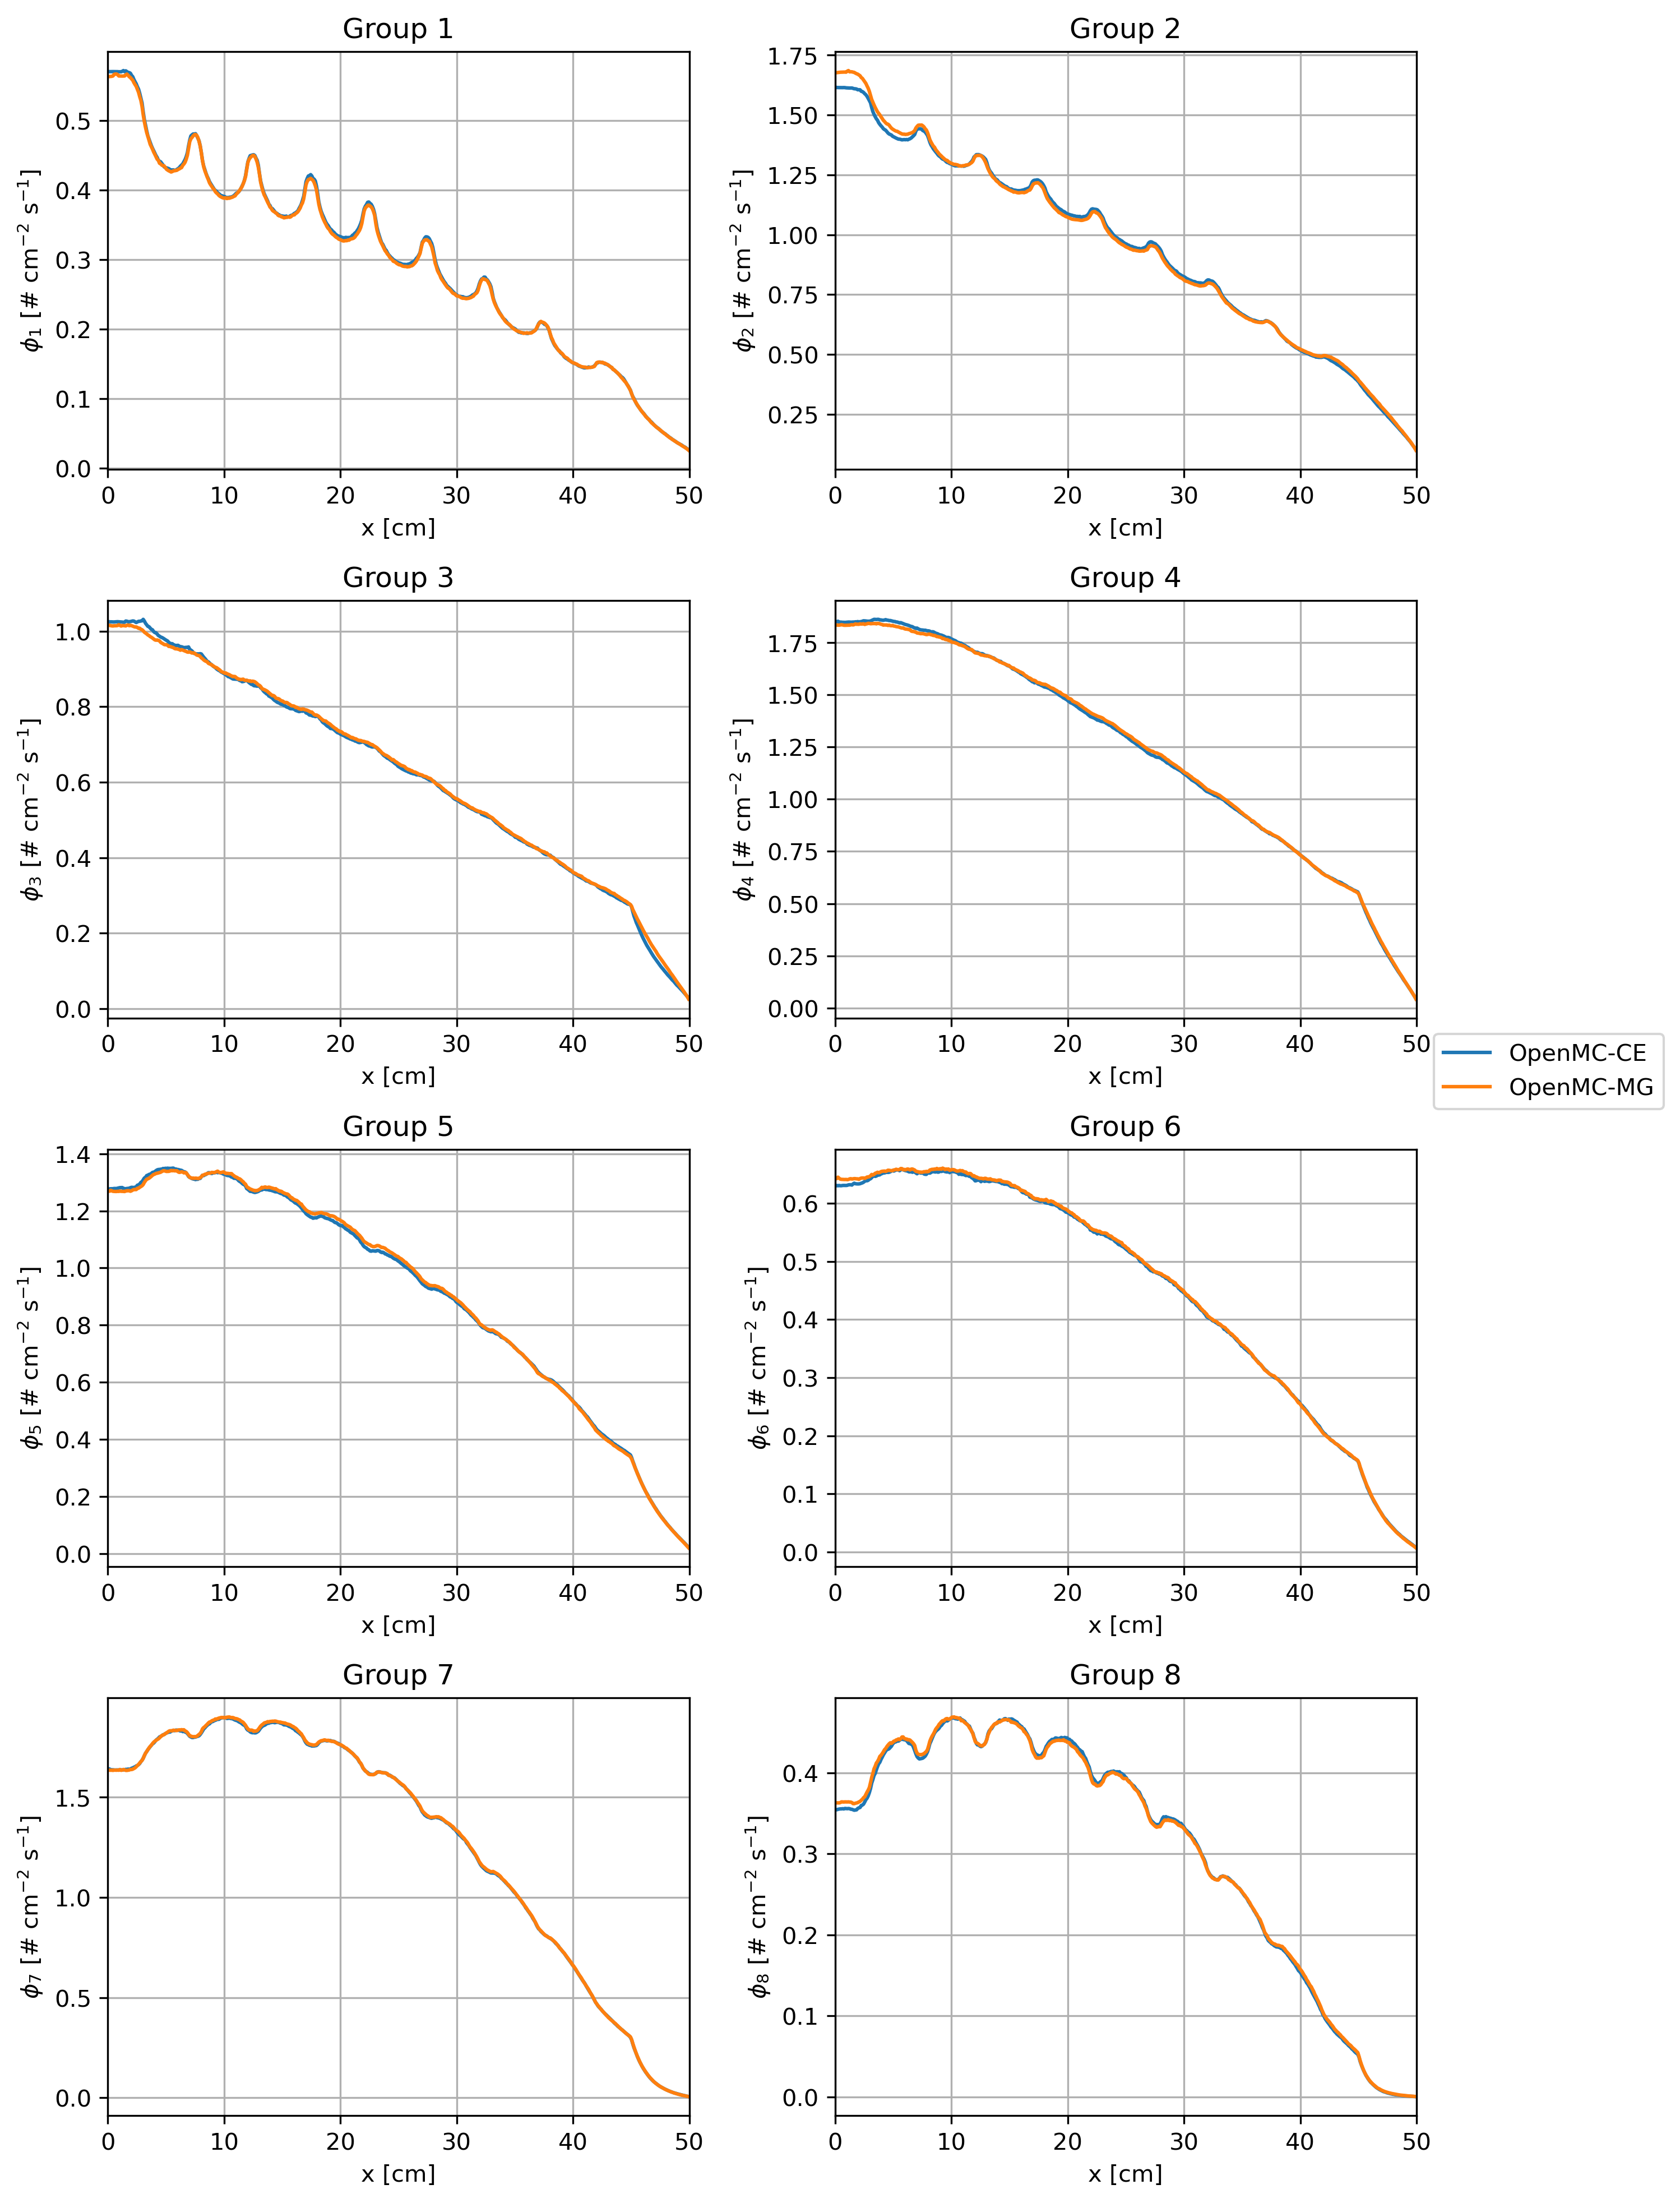
\includegraphics[width=\columnwidth]{case-3a-flux}
      \caption{Case 3a neutron group flux distributions from OpenMC-CE and OpenMC-MG.}
      \label{fig:3a-flux}
    \end{figure}
    \column{5.5cm}
    \begin{figure}[htb!]
      \centering
      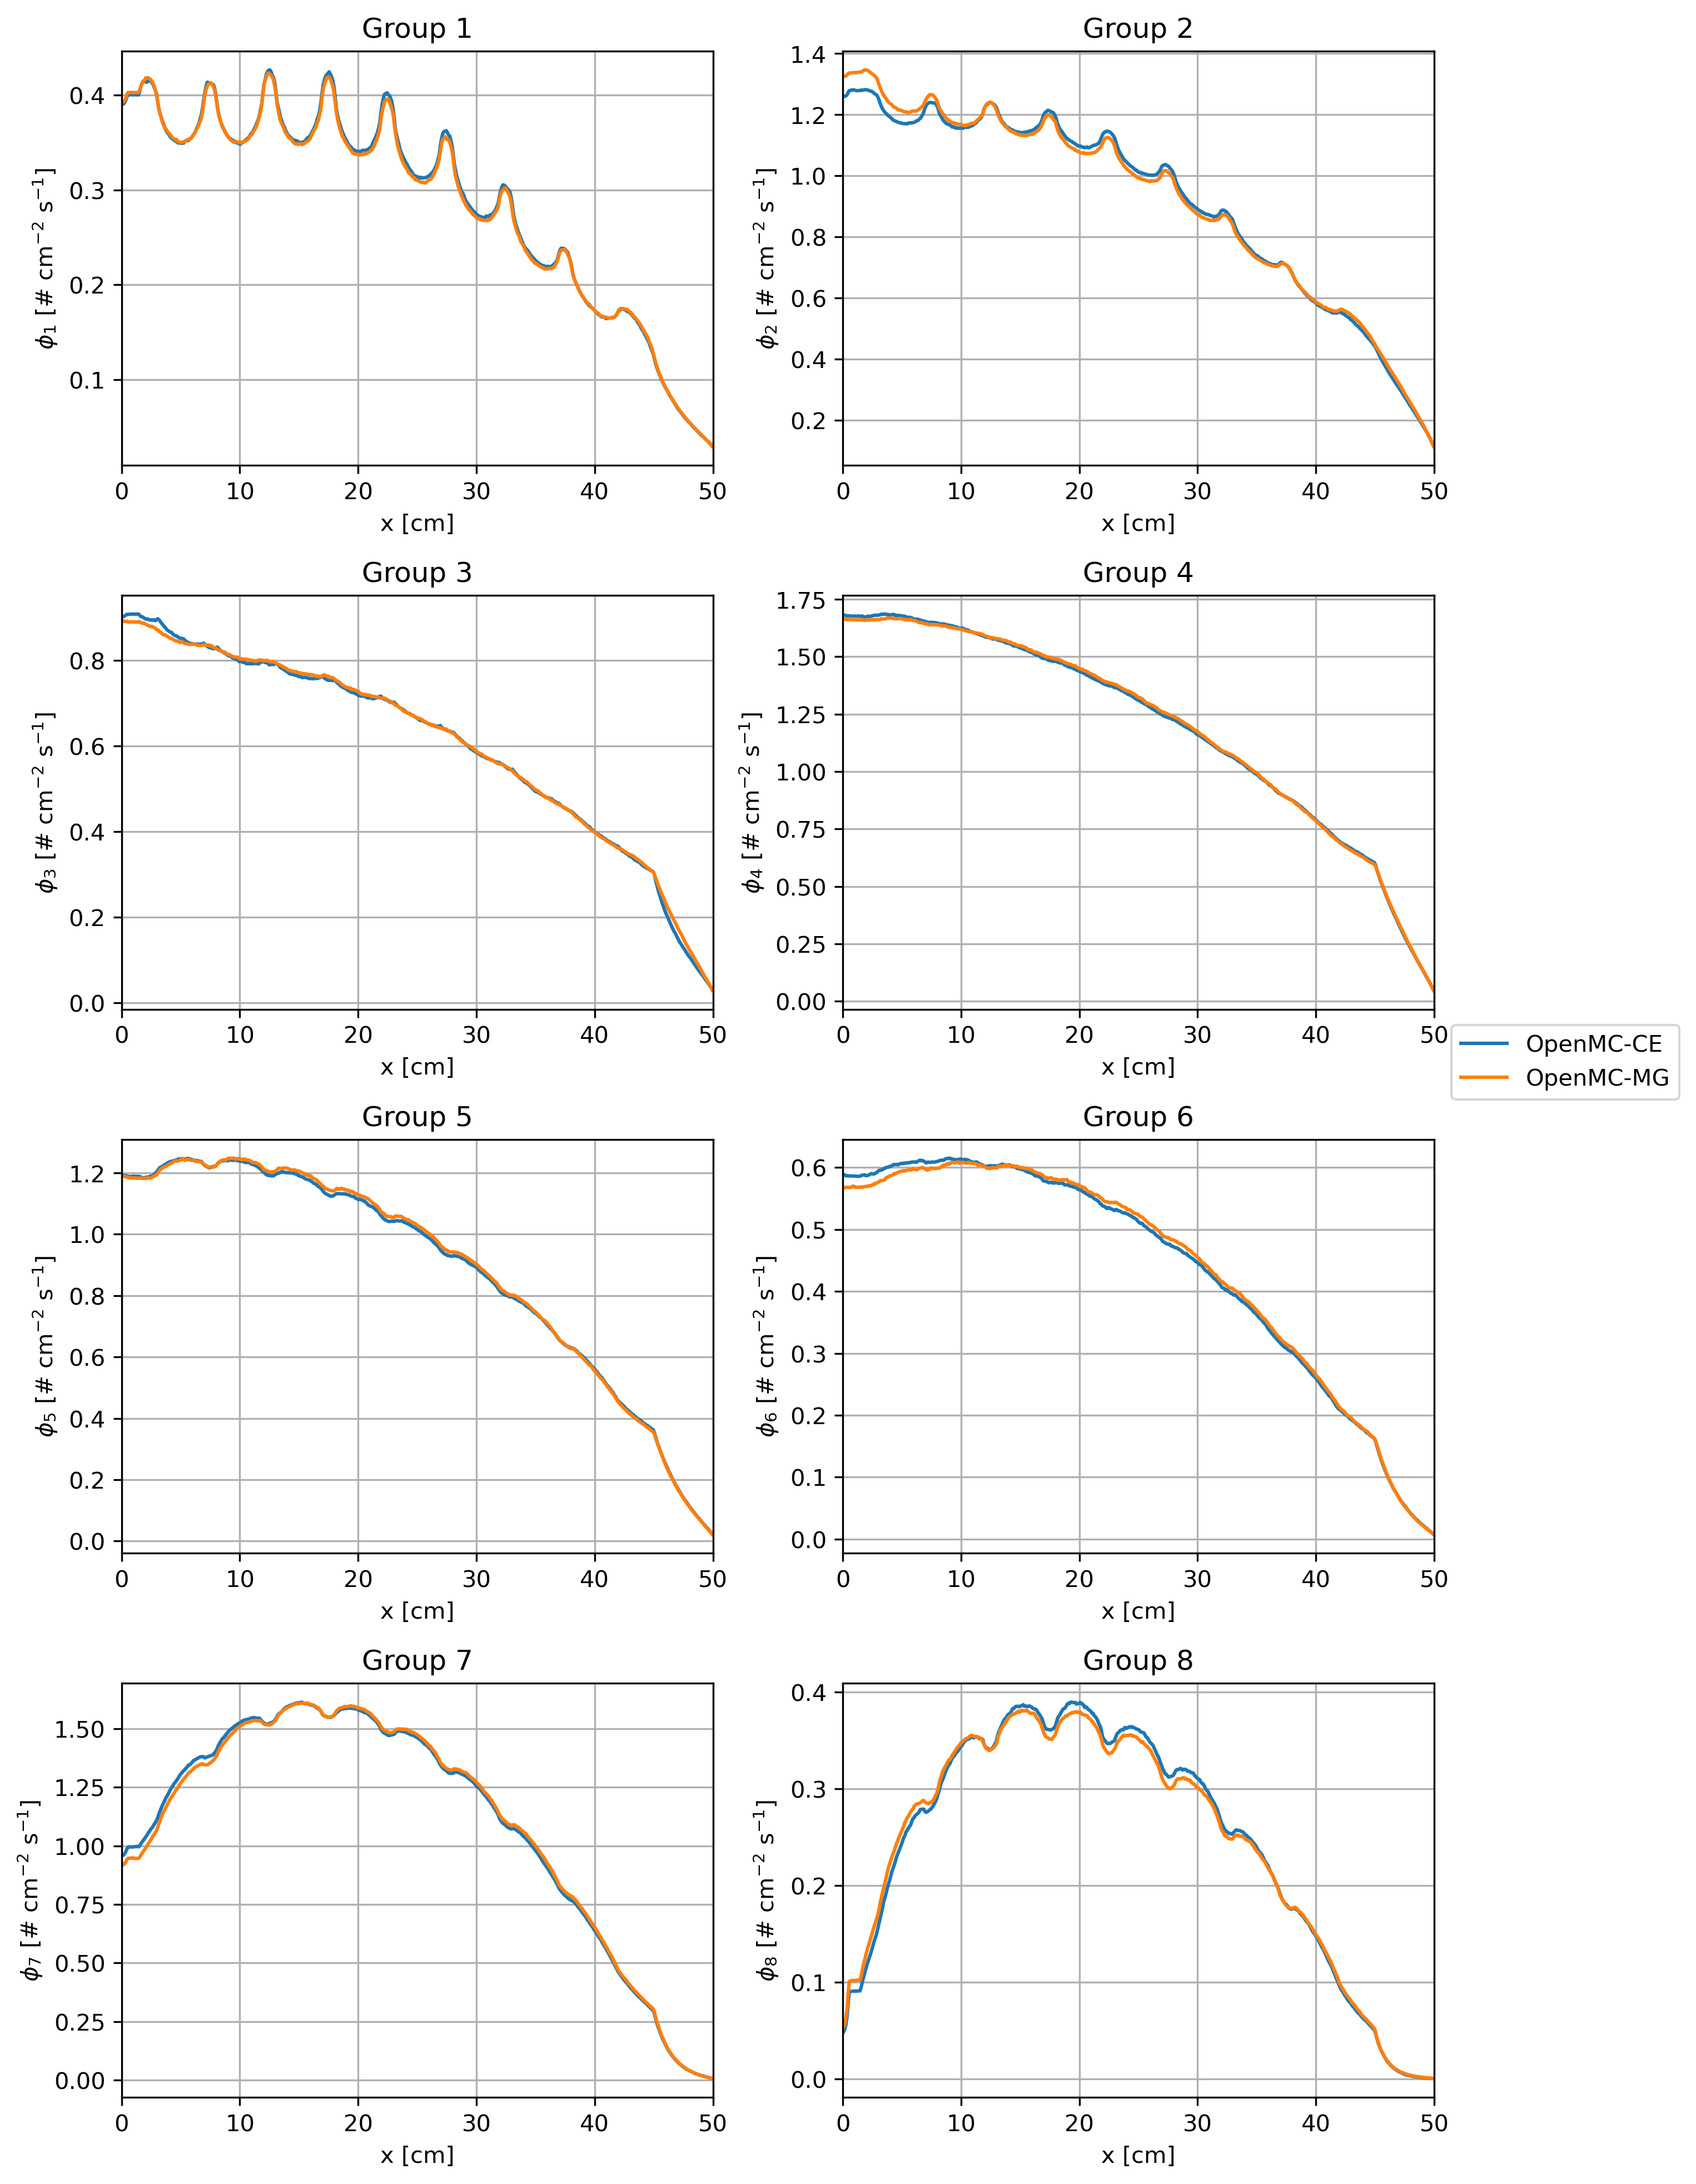
\includegraphics[width=\columnwidth]{case-3b-flux}
      \caption{Case 3b neutron group flux distributions from OpenMC-CE and OpenMC-MG.}
      \label{fig:3b-flux}
    \end{figure}
  \end{columns}
\end{frame}

\begin{frame}
%  \frametitle{Hybrid $S_N$-Diffusion Method: 1-D Neutronics Eigenvalue Simulations}
  \begin{columns}
    \column{5.5cm}
    \textbf{Case 3a Neutron Flux Distributions}
    \begin{itemize}
      \item The neutron diffusion and hybrid methods fare worse than the $S_8$ method at capturing
        the oscillatory flux pattern.
      \item The hybrid method performs better than the neutron diffusion method near $x=0$ cm where
        the correction region is situated.
    \end{itemize}
    \column{5.5cm}
    \begin{figure}[htb!]
      \centering
      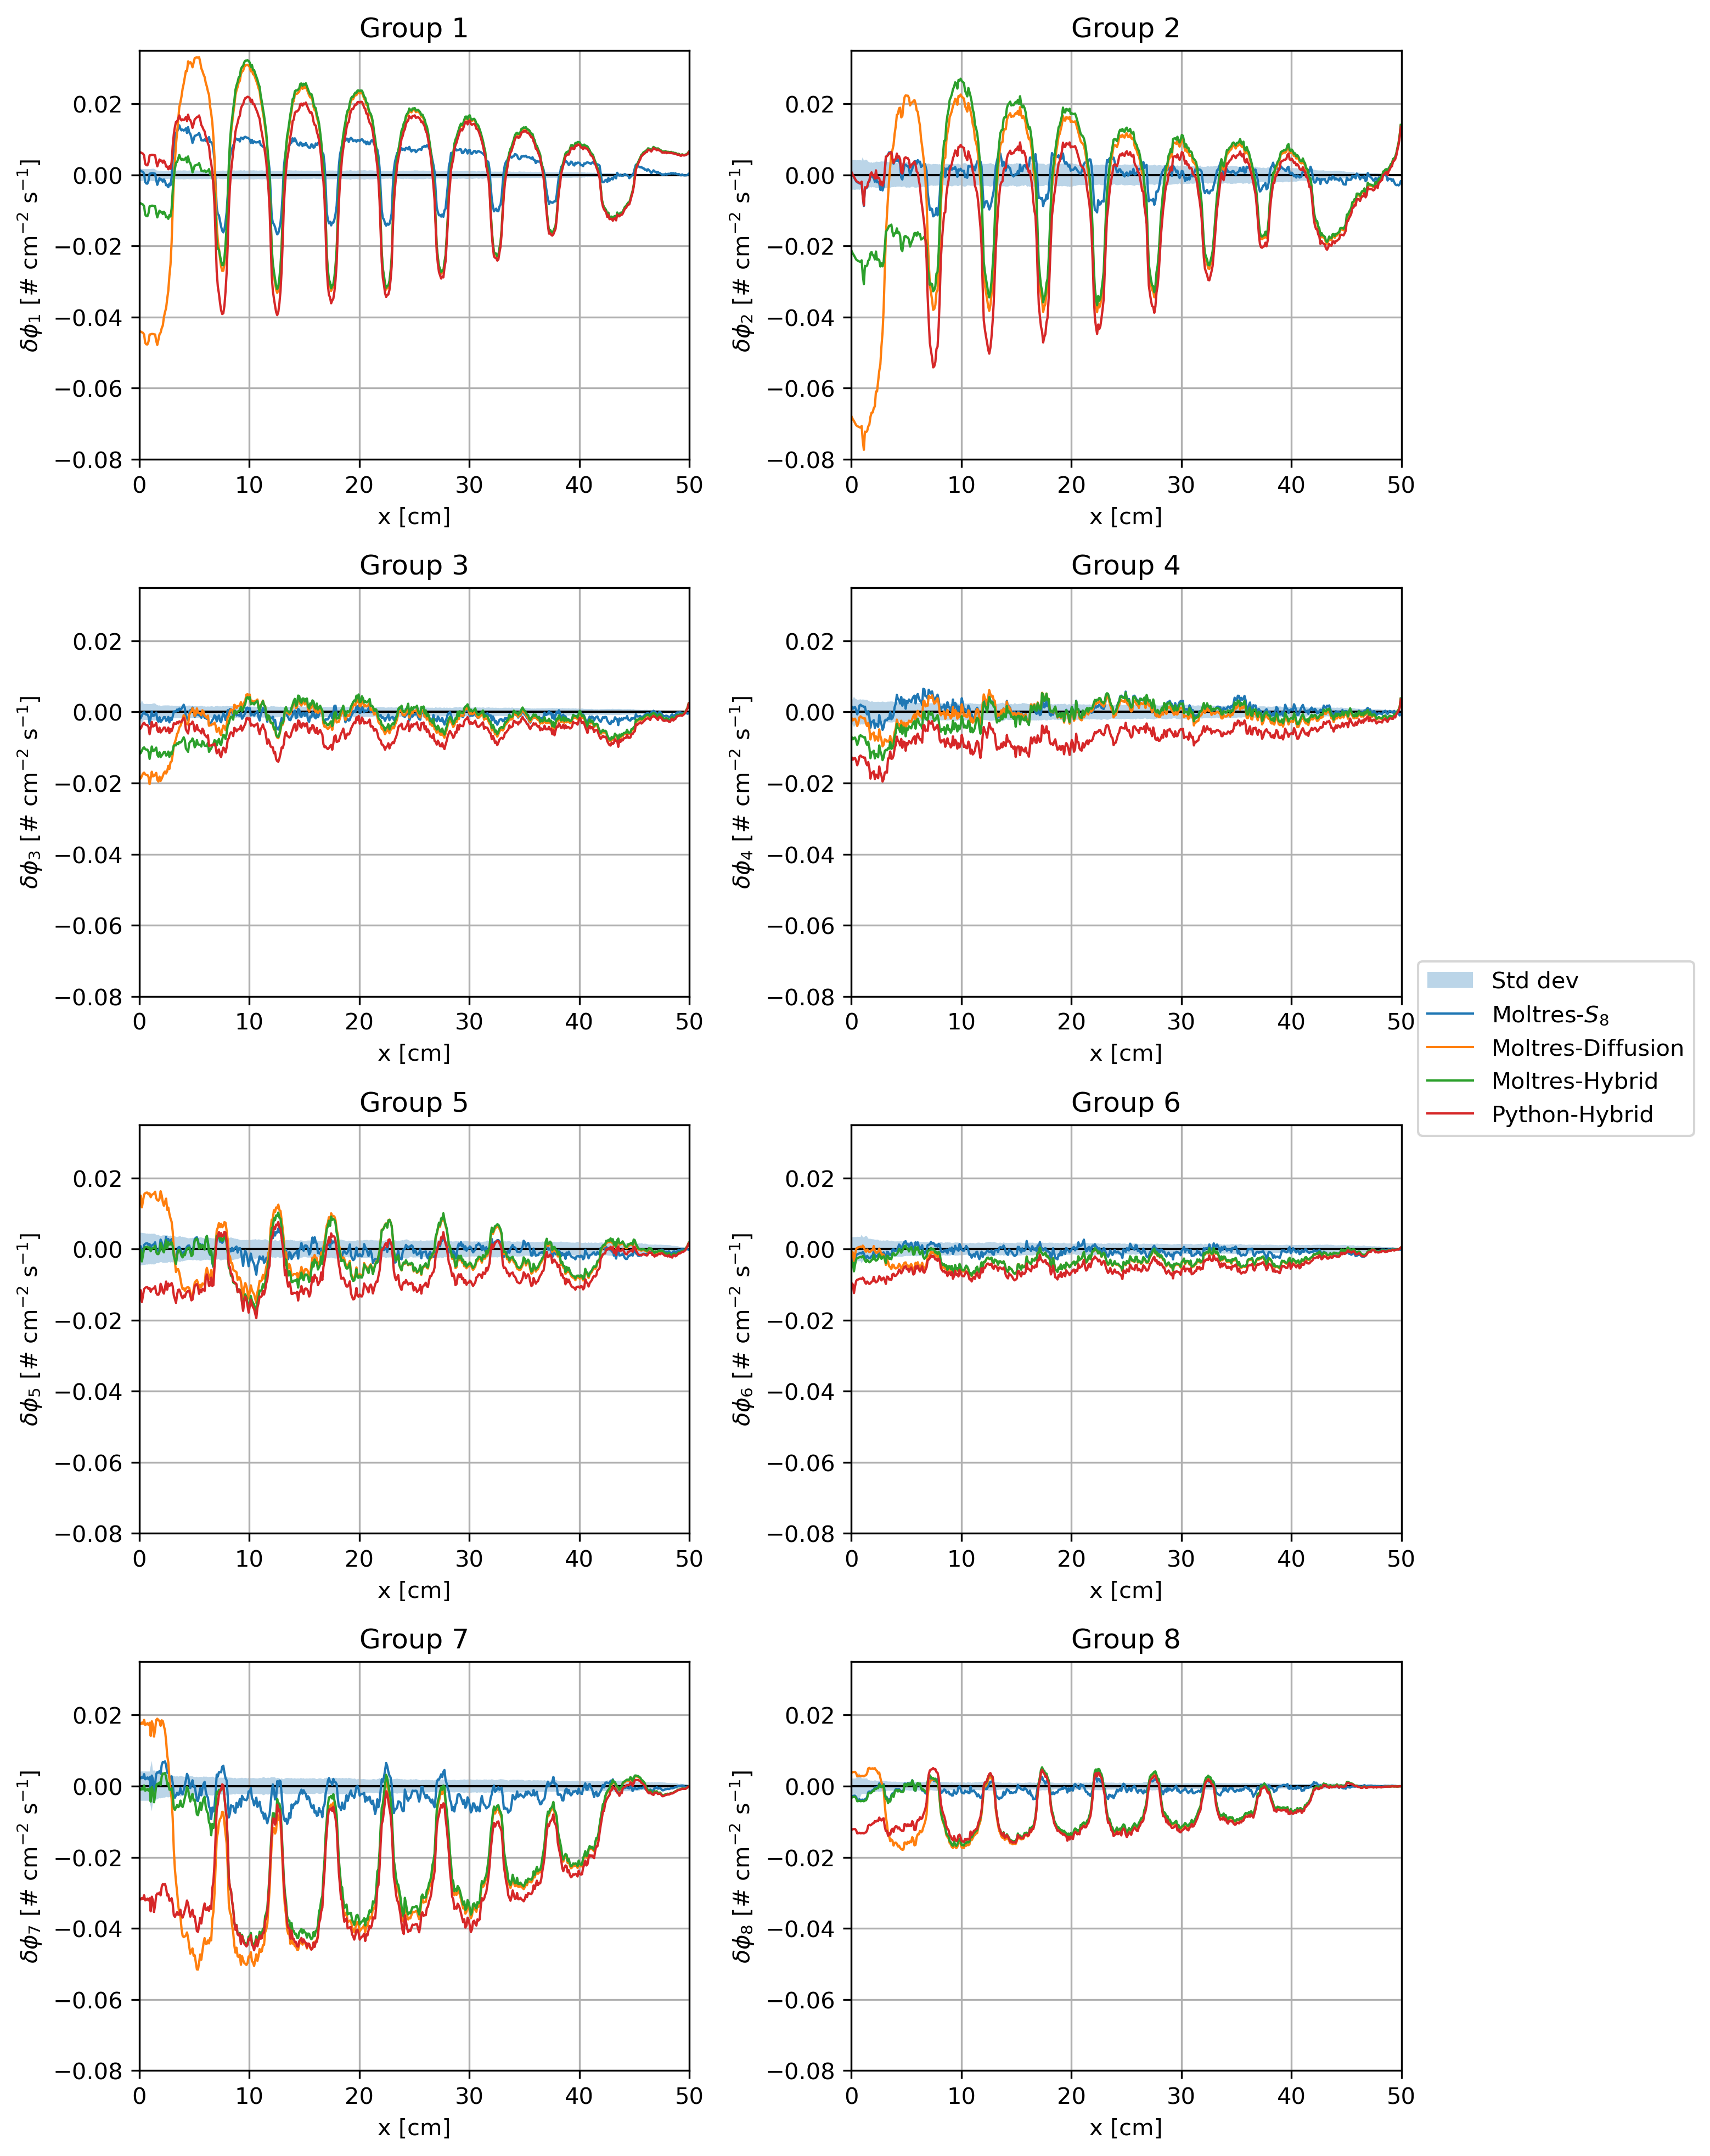
\includegraphics[width=.975\columnwidth]{case-3a-flux-diff}
      \caption{Absolute difference in neutron group flux distributions for Case 3a from Moltres-$S_8$,
      Moltres-diffusion, Moltres-hybrid, and Python-hybrid relative to OpenMC-MG.}
      \label{fig:3a-flux-diff}
    \end{figure}
  \end{columns}
\end{frame}

\begin{frame}
%  \frametitle{Hybrid $S_N$-Diffusion Method: 1-D Neutronics Eigenvalue Simulations}
  \begin{columns}
    \column{5.5cm}
    \textbf{Case 3b Neutron Flux Distributions}
    \begin{itemize}
      \item The neutron diffusion method performance worsens with the control rod region introduced
        near $x=0$.
    \end{itemize}
    \column{5.5cm}
    \begin{figure}[htb!]
      \centering
      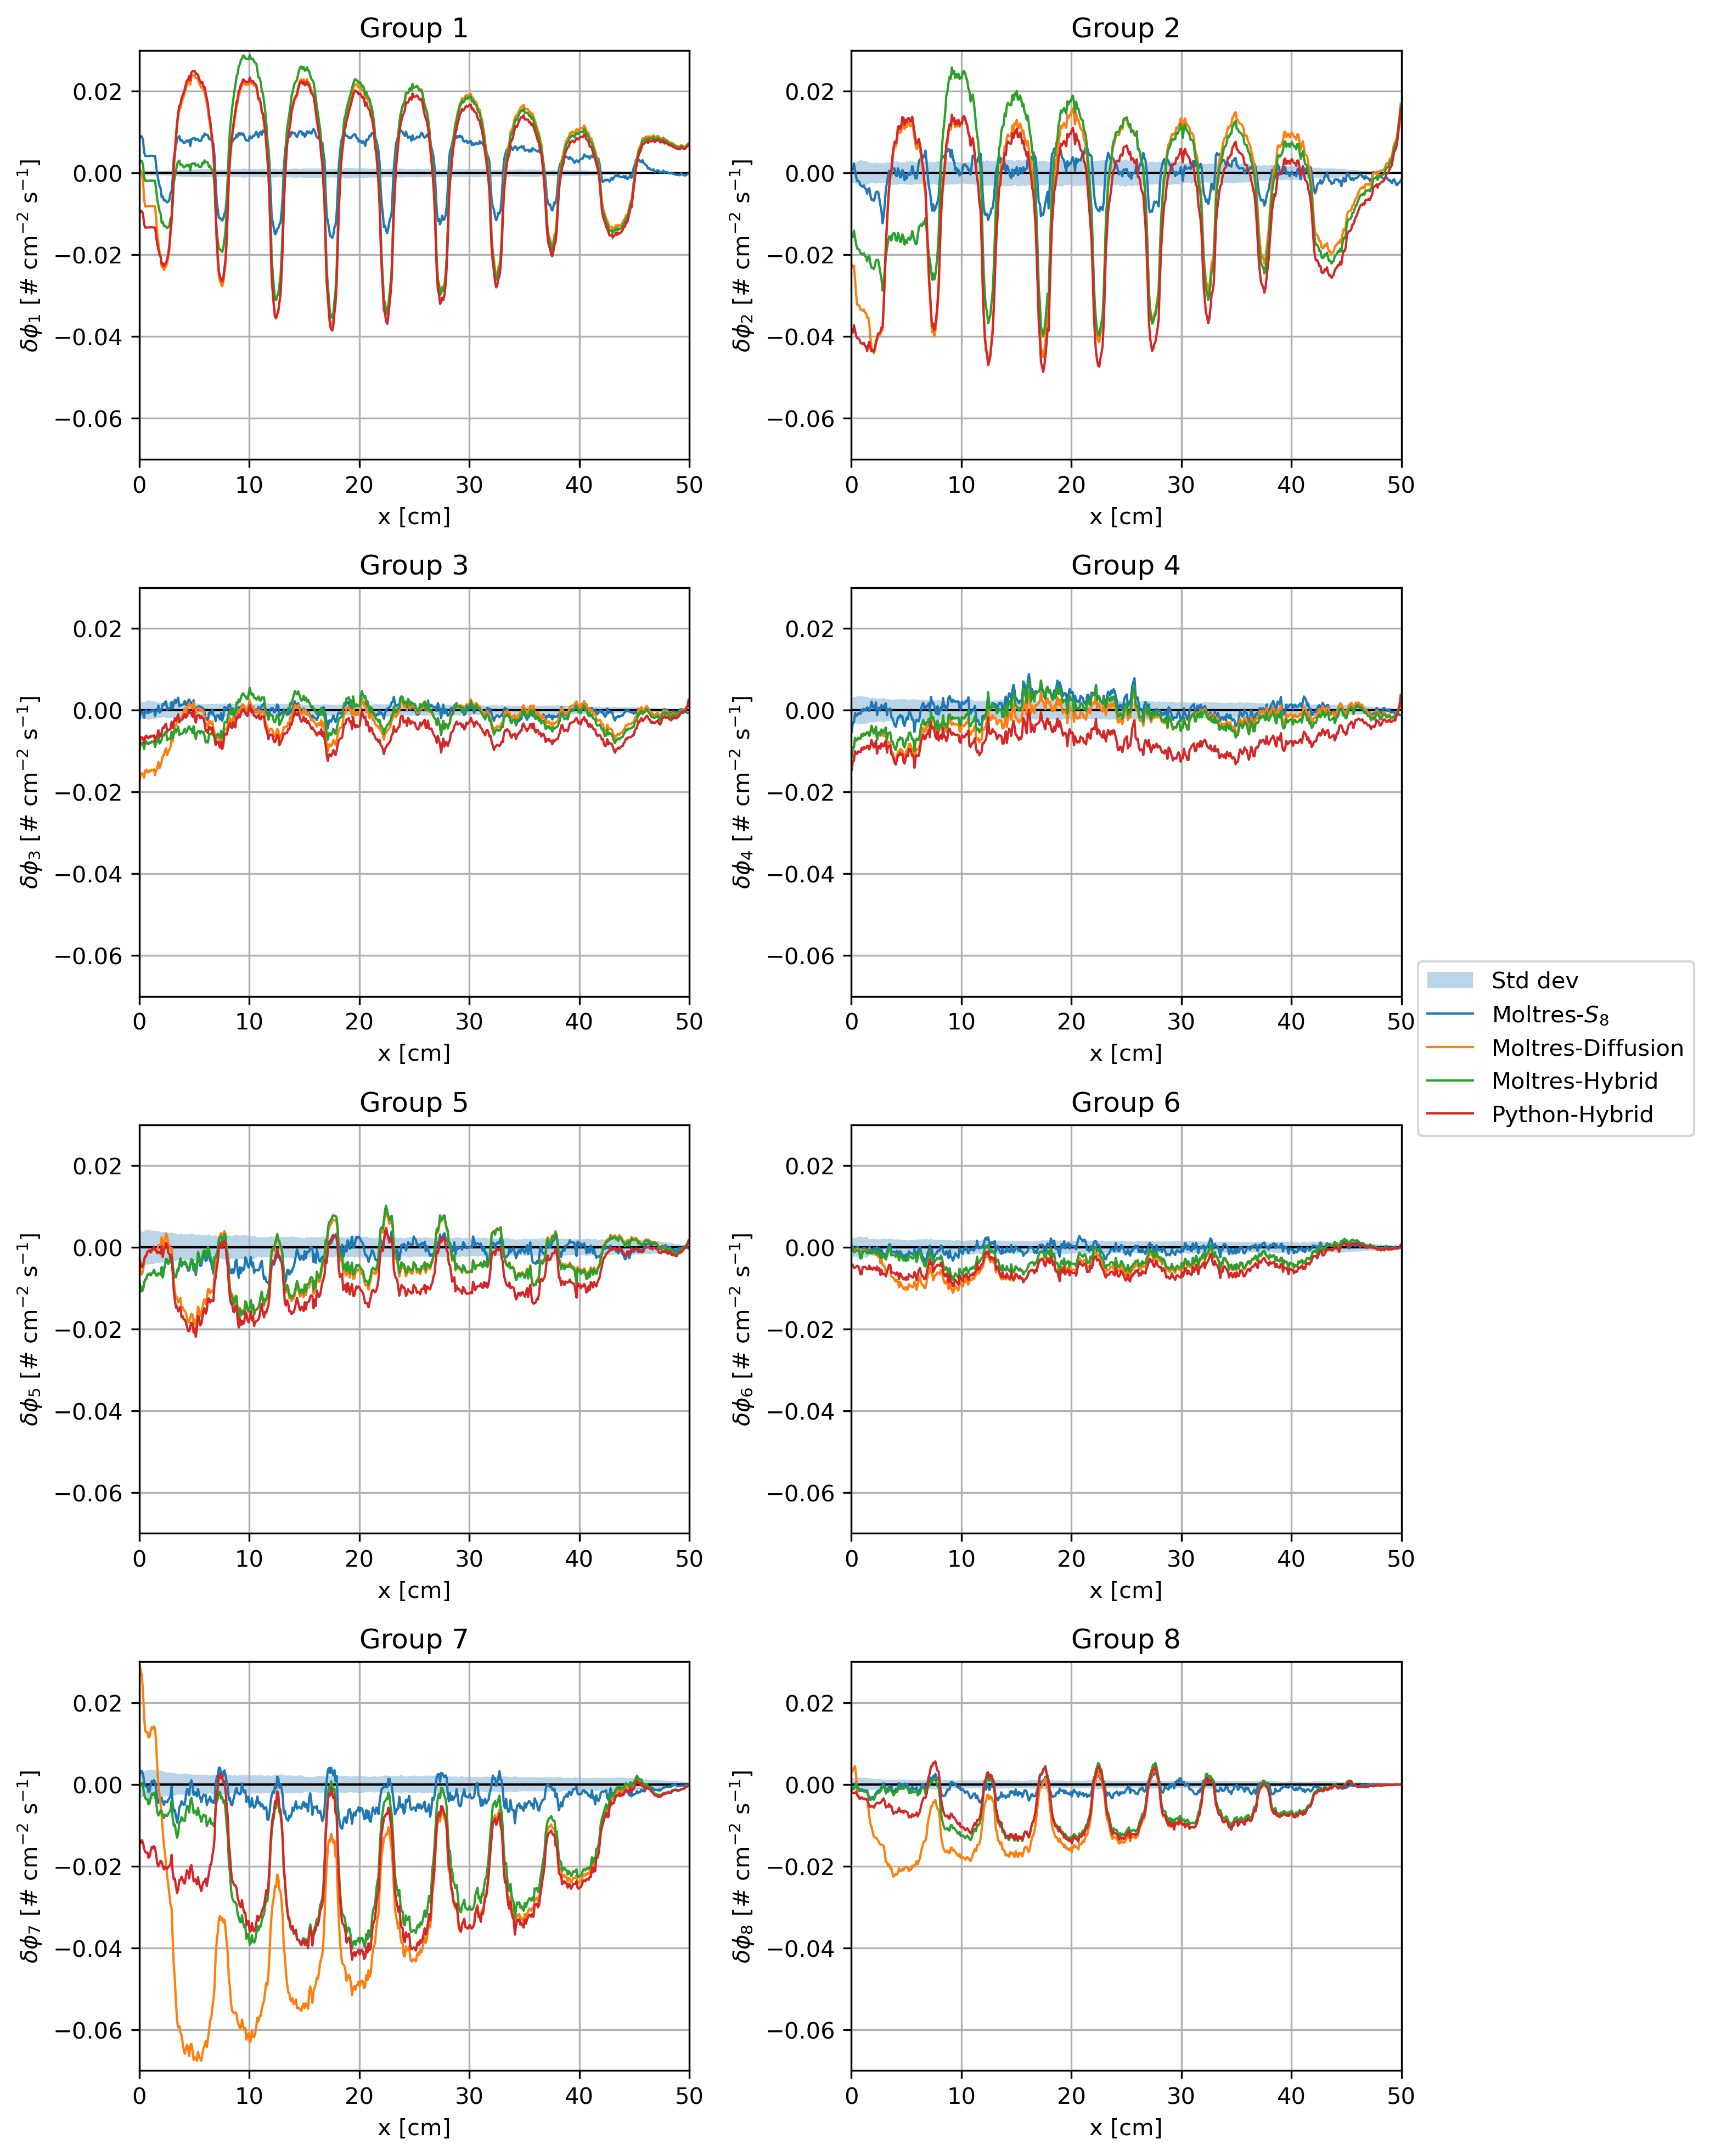
\includegraphics[width=.975\columnwidth]{case-3b-flux-diff}
      \caption{Absolute difference in neutron group flux distributions for Case 3b from Moltres-$S_8$,
      Moltres-diffusion, Moltres-hybrid, and Python-hybrid relative to OpenMC-MG.}
      \label{fig:3b-flux-diff}
    \end{figure}
  \end{columns}
\end{frame}

\begin{frame}
  \frametitle{Hybrid $S_N$-Diffusion Method: 1-D Neutronics Eigenvalue Simulations}
  \textbf{Impact of Correction Subregion Sizes on $k$}
  \begin{itemize}
    \item Minimizing the correction region size is essential for the hybrid method to be
      computationally efficient for time-dependent simulations.
    \item $k$ varies by up to 164 pcm for Case 3a and 109 pcm for Case 3b.
    \item The hybrid method $k$ value does not converge monotonically towards the $S_8$ method $k$ value,
      implying other sources of discrepancies.
  \end{itemize}
  \begin{figure}[h]
    \centering
    \begin{subfigure}[b]{0.49\columnwidth}
      \centering
      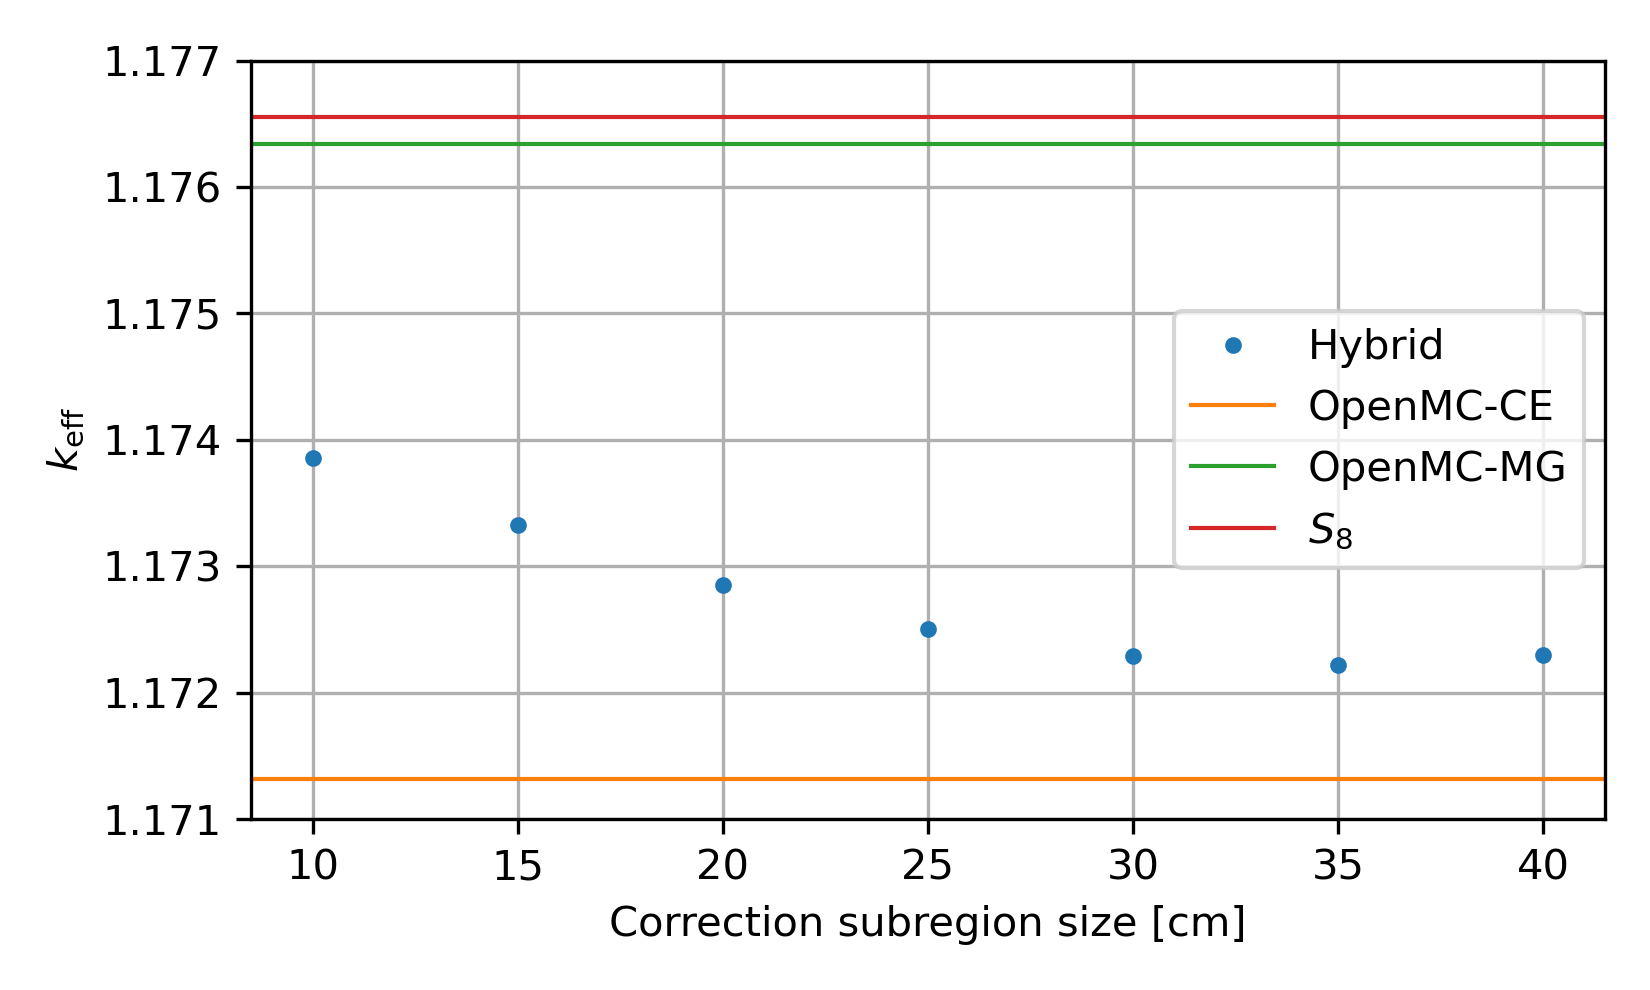
\includegraphics[width=\columnwidth]{correction-size-a-k}
      \caption{Case 3a}
      \label{fig:v1-size-a-k}
    \end{subfigure}
    \hfill
    \begin{subfigure}[b]{0.49\columnwidth}
      \centering
      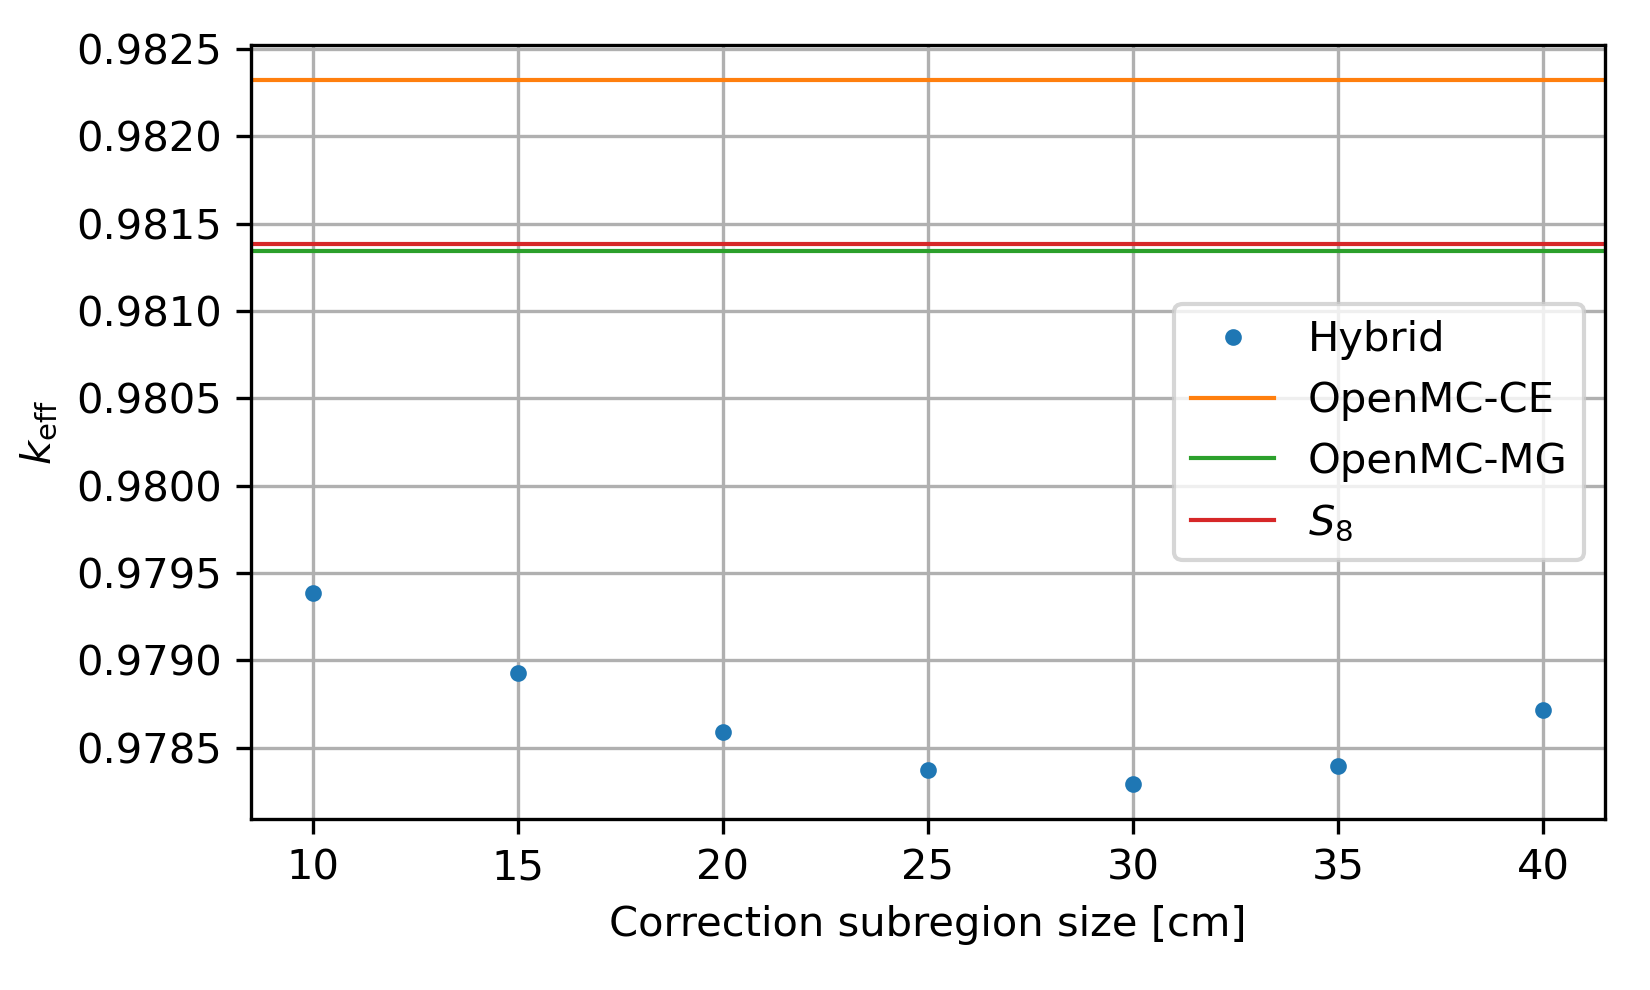
\includegraphics[width=\columnwidth]{correction-size-b-k}
      \caption{Case 3b}
      \label{fig:v1-size-b-k}
    \end{subfigure}
    \caption{$k_\text{eff}$ estimates from the hybrid method for Cases 3a and 3b with different
    correction subregion sizes. The horizontal lines indicate $k_\text{eff}$ estimates from the
    OpenMC-CE, OpenMC-MG, and $S_8$ methods.}
    \label{fig:v1-size-k}
  \end{figure}
\end{frame}

\begin{frame}
  \frametitle{Hybrid $S_N$-Diffusion Method: 1-D Neutronics Eigenvalue Simulations}
  \textbf{Impact of Correction Subregion Sizes on Rod Worth}
  \begin{itemize}
    \item Rod worth estimates vary non-monotonically with increasing correction subregion size.
    \item Rod worth estimates remain within 0.2 \% of the $S_8$ method rod worth.
    \item The hybrid method produces accurate rod worth estimates as long as the correction region
      size is kept consistent.
  \end{itemize}
  \begin{figure}[htb!]
    \centering
    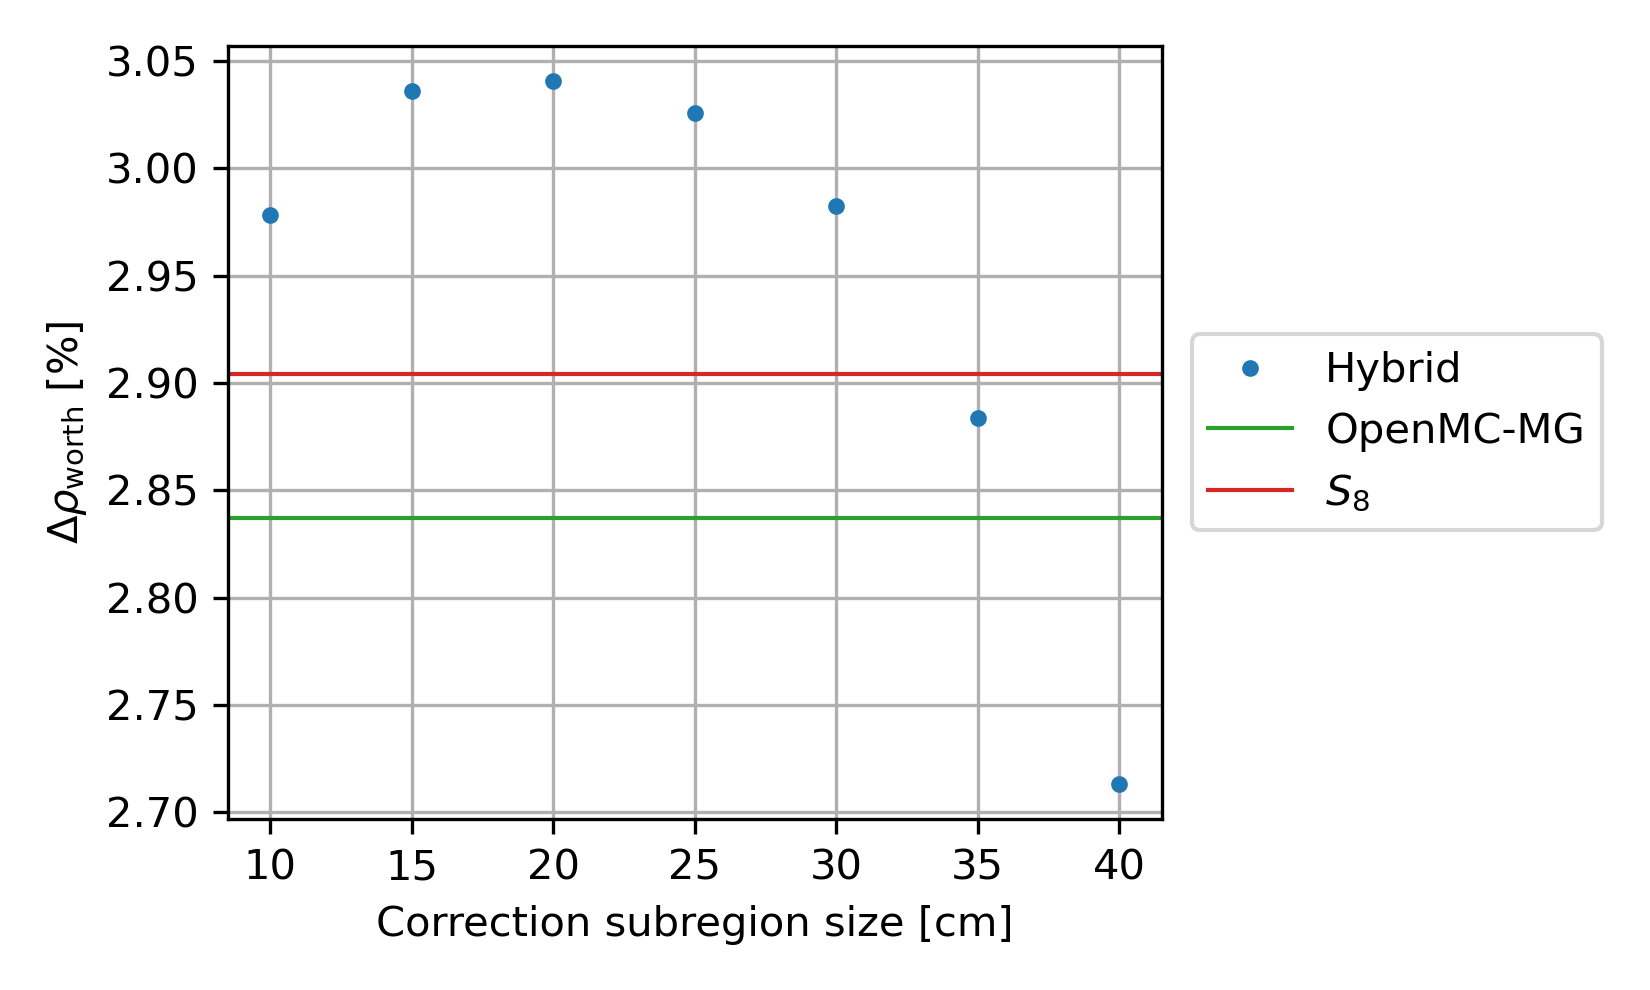
\includegraphics[width=0.6\columnwidth]{correction-size-rho}
    \caption{Percentage difference in rod worth from the hybrid method relative to OpenMC-CE for
      Cases 3a and 3b with different correction subregion sizes. The horizontal lines indicate
      equivalent rod worth differences from the OpenMC-MG and $S_8$ methods.}
    \label{fig:v1-size-rho}
  \end{figure}
\end{frame}

\begin{frame}
  \frametitle{Hybrid $S_N$-Diffusion Method: 1-D Neutronics Eigenvalue Simulations}
  \textbf{Relaxing the $S_N$ Convergence Tolerance}
  \begin{itemize}
    \item The hybrid $S_N$-diffusion method iteratively couples the neutron diffusion solver with
      the $S_N$ subsolver.
    \item Diffusion-based acceleration schemes for neutron transport methods typically do not
      require the neutron transport calculations to fully converge.
    \item Transport correction parameters tend to converge faster than scalar flux.
    \item Relaxing the $S_N$ subsolver convergence tolerance would provide computational savings to
      the hybrid method.
  \end{itemize}
\end{frame}

\begin{frame}
  \frametitle{Hybrid $S_N$-Diffusion Method: 1-D Neutronics Eigenvalue Simulations}
  \begin{columns}
    \column{7cm}
    \textbf{Relaxing the $S_N$ Convergence Tolerance}
    \begin{itemize}
      \item The number of outer iterations generally increases with the $S_8$ convergence tolerance.
      \item The hybrid method exhibits superlinear ($q=1.333$) convergence in $k$ with respect to
        the $S_8$ convergence tolerance value.
    \end{itemize}
    \begin{table}[h]
      \centering
      \caption{Number of outer iterations in hybrid method calculations of Case 3b for a given set of
      convergence tolerance values imposed on the $S_8$ subsolver.}
      \small
      \setlength\tabcolsep{2pt}
      \begin{tabular}{l S S S S S S}
        \toprule
        $S_8$ subsolver tolerance, $\epsilon_\text{tol}$ & {$10^{-8}$} & {$10^{-7}$} & {$10^{-6}$} & {$10^{-5}$} & {$10^{-4}$} & {$10^{-3}$} \\
        \midrule
        Number of outer iterations & 3 & 3 & 3 & 2 & 2 & 1 \\
        \bottomrule
      \end{tabular}
      \label{table:sn-tol}
    \end{table}
    \column{4cm}
    \begin{figure}[h]
      \centering
      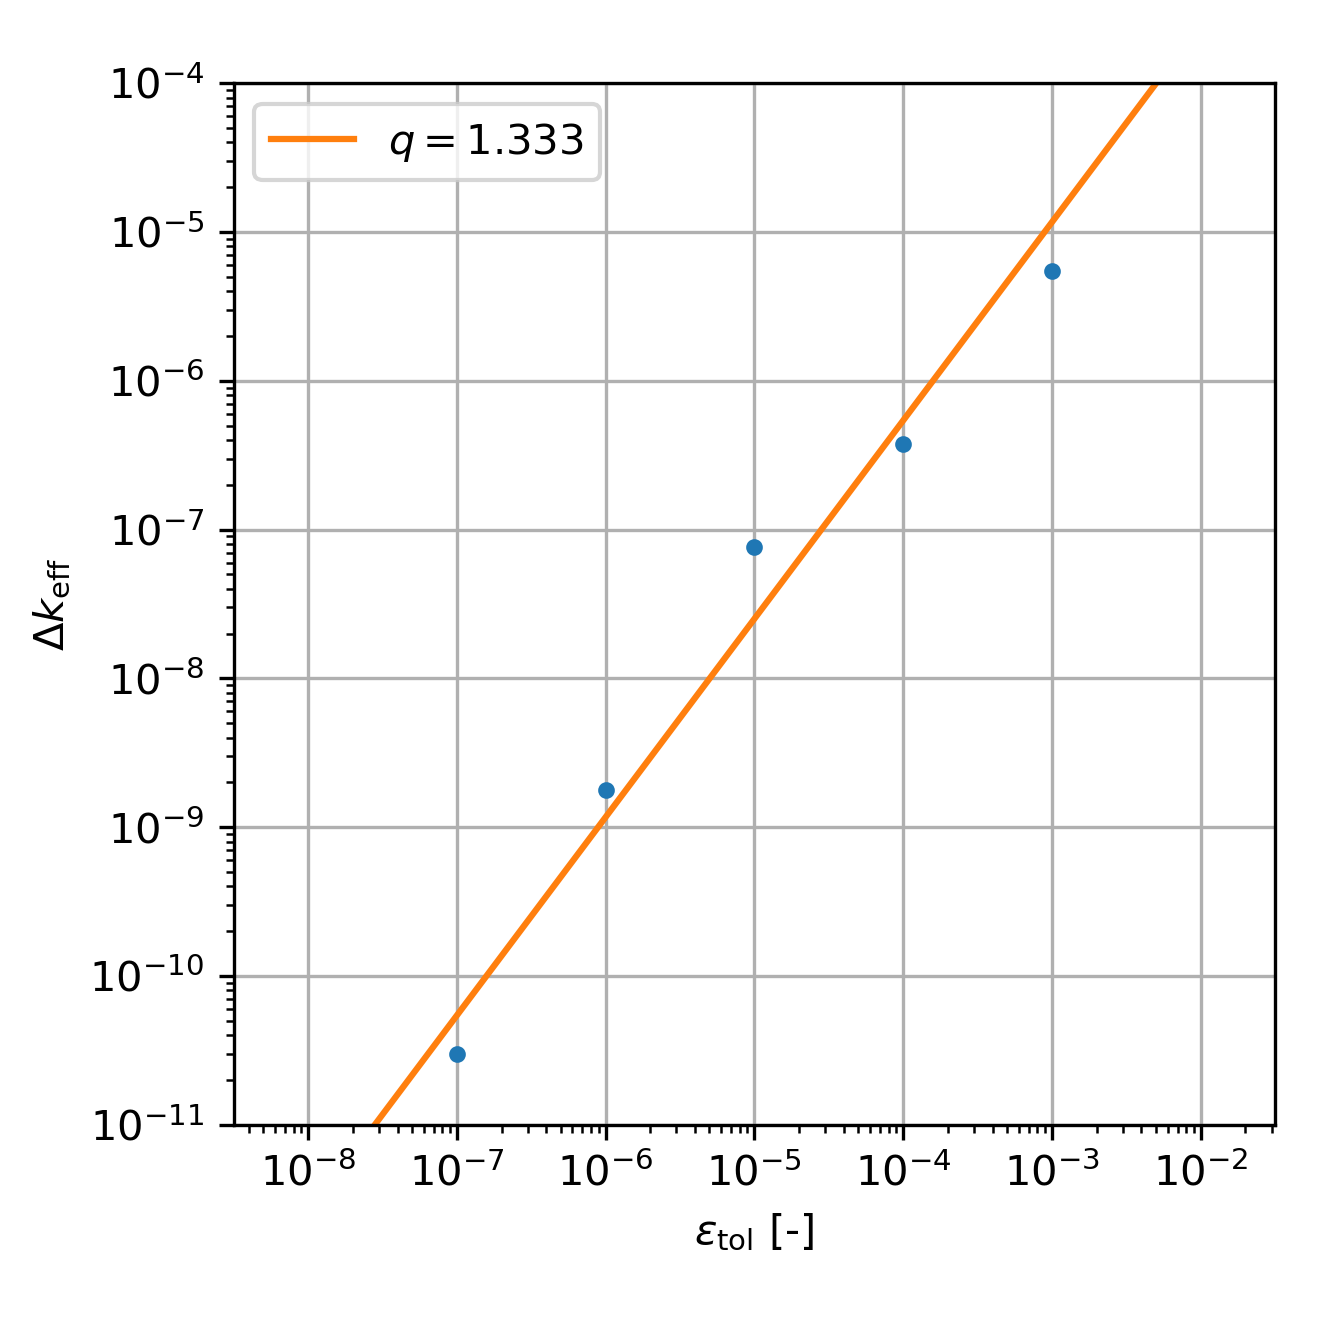
\includegraphics[width=\columnwidth]{sn-tol}
      \caption{$k_\text{eff}$ error estimates of Case 3b for a range of convergence tolerance values
      imposed on the $S_8$ subsolver relative to the reference $k_\text{eff}$ value when
      $\epsilon_\text{tol}=10^{-8}$.}
      \label{fig:sn-tol}
    \end{figure}
  \end{columns}
\end{frame}
